\documentclass{article}

\usepackage{graphicx}
\usepackage{hyperref}
\usepackage[utf8]{inputenc}

\title{Relatório da segurança do SSL sobre dados}
\author{Nalbert Gabriel Melo Leal}
\date{13-10-2017}

\begin{document}

  \pagenumbering{gobble}

  \begin{figure}
		
\includegraphics[width=\textwidth]{imdLogo.png}
		\label{fig:imdLogo}
	\end{figure}

  \maketitle

  \newpage

  \tableofcontents
  \newpage

  \pagenumbering{arabic}

  \section{Introdução}

  \newpage

  \section{SSL}
  \subsection{Oque é SSL ?}
  \paragraph{}
  No ano de 1994 a Netscape criou um protocolo de segurança chamado SSL (secure
  socket layer) que cria um tunel lógico entre dois comutadores para que a
  comunicação entre eles não possa ser conpreendida por terceiros. Entenda o
  tunel lógico como uma comunicação sendo feita com uso de criptografia.
  \paragraph{}
    Esse canal criptografado entre é muito utilizado nos dias de hoje entre
  servidores e clientes para aumentar a segurança durante a troca de dados.
  Durante o acesso a um site para saber se existe o uso de SSL basta verificar
  se ao lado da URL da pagina existe o simbolo de um cadeado fechado, indicando
  uma conexão segura.

  \subsection{Como o SSL funciona ?}
  \paragraph{}
  O SSL como protocolo é bem simples. Para ativar o SSL em um sevidor é
  nescessário responder a algumas questões sobre identidade de quem esta sendo
  certificado (o servidor) e assim gerar um certificado que apos algum tempo
  definido irá ser invalidado.
  \paragraph{}
    Quando um servidor é requisitado por um cliente ele usa o certificado gerado
  para criar uma chave privada e uma publica. A chave privada vai servir para
  descriptografar os dados vindos do cliente, já a chave publica server para o
  cliente ter certza que a informação vem do servidor. Essas duas chaves permitem
  a troca de chaves unicas para que a comunicação atravez do canal criptografado
  possa acontecer.

  \subsection{É o SSL a prova de hackers ?}
    Já mencionamos que o SSL foi desenvolvido para aumentar a segurança entre
  cliente e servidor, entretanto isso não significa que seja inpossivel de
  burlar ou de descriptografar. Com pesquisas e com a insistencia de hackers é
  comum que em algum mommento se descubra vulnerabilidades.
  \paragraph{}
    No caso do SSL existe maneiras de se interceptar a comunicação no momento
  que ela esta sendo iniciada e assim interceptar os dados da comunicação. Esse
  metodo de invasão é chamado de "man in the middle", traduzido para "o homem
  no meio".
  \paragraph{}
    Esse ataque é potencialmente perigoso e permite que um atacante possa
  descobrir dados sensiveis de usuarios/servidor, sendo assim vamos demonstrar
  o quanto é fácil fazer um ataque "man in the middle" e como ele pode ser
  devastador, tanto para o usuário que pode ser colocado em grande risco e
  para o servidor, pois a baixa segurança pode fazer o numero de usuários cair.

  \newpage

  \section{Problemas do SSL}
  \paragraph{}
    Discutimos brevemente na sessão anterior um ataque que pode ocorrer ao SSL,
  mas esse não é o unico problema envolvendo o uso do SSL.

  \subsection{Prpblemas do SSL}
  \paragraph{}
  Se olharmos esse protocolo por sí só podemos achar que os motivos para não
  usa-lo são fracos, entretanto após olharmos um acumulo desse motivos podemos
  acabar vendo se vale ou não a pena usar.

  \begin{enumerate}
    \item O SSL causa um incremento no custo conputacional. Isso ocorre pois
    esse protocolo faz uso de criptografia, e a criptografia requer que sejam
    usados algoritimos custosos para encriptar e desencriptar.
    \item Aparentemente o SSL inpede que alguns tipos de cache, por exemplo o
    proxy transparente de ISP (Internet Service Provider ou em português
    Provedor de Serviço Internet). Com isso é nescessário um aumento no consumo
    de banda do servidor.
  \end{enumerate}

  \subsection{Como funcioan o ataque "man in the middle" ?}
  \paragraph{}
    Em uma coneção normal de troca e informações dois computadores trocam dados
  sem a interferência de terceiros. O termo "man in the middle" é uma referência
  a um ataque em que o atacante intercepta os dados entre duas pessoas (por
  exemplo o usuário e o facebook), registra esses dados e em alguns casos até
  os altera sem que as vítimas percebam.
  \paragraph{}
    Esse ataque claramente é extremamente perigoso por conta do atacante ter
  acesso aos dados que estão criptografados. Ocorre da seguinte forma:

  \begin{enumerate}
    \item O usuário faz uma requisição a um servidor.
    \item O atacante finge que é o servidor e assim intercepta a requisição.
    \item O atacante tem acesso aos dados do usuário em texto limpo.
    \item com esses dados pode-se fazer uma requisição ao servidor e receber
    a resposta.
    \item envia a resposta de volta ao usuario.
    \item usuário recebe a resposta e pensa que está em uma conexão segura.
  \end{enumerate}

  \subsection{O ataque "Man in the middle" e o SSL}
  \paragraph{}
  Como foi visto esse ataque é facil de se entender, a maneira como ele
  funciona com o SSL é igual com modificações para que o ataque funcione nesse
  protocolo. Com o SSL o atacante ao interceptar a conexão força um "downgrade"
  do HTTPS (HTTP sobre SSL) para HTTP e assim tem acesso aos dados do cliente
  em texto limpo, com isso pode fazer a conexão com o servidor e retornar a
  resposta ao usuário. Abaixo uma imagem:

  \begin{figure}[h!]
		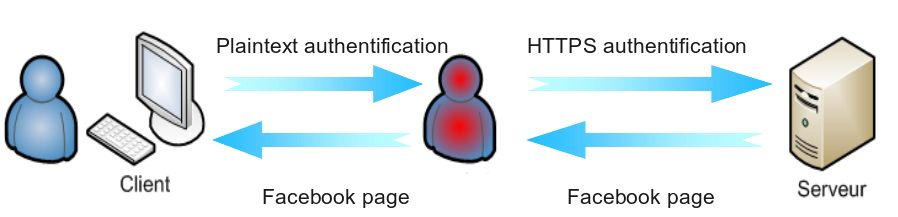
\includegraphics[width=\textwidth]{httpsManInTheMiddle.png}
		\label{fig:httpsManInTheMiddle}
	\end{figure}

    Na proxima sessão tem um passo-a-passo de como fazer o um ataque
  "man in the middle" e assim demonstrar que é um ataque completamente de
  ser executado com um conhecimento extremamente básico de redes de computadores
  possivel.

  \newpage

  \section{O experimento}
    Nessa sessão vamos demonstrar o quão facil é para interceptar dados SSL e
  assim ter acesso a dados dos usuários. Será tanbém demonstrado que o nivel de
  conhecimento nescessário é muito baixo, visto que usaremos ferramentas já prontas,
  assim podemos dizer que "lamers" podem facilmente fazer esse ataque, mostrando
  ser um ataque que nas mãos de hackers experientes pode acabar causando grandes
  danos ao serviço.

  \subsection{Requisitos}
    Os requisitos para fazer o experimento são os mesmos utilizados na hora
  da montagem para garantir que não averá problemas quando for replicado pelo
  leitor.

    \begin{enumerate}
      \item Possuir três computadores com o  sistema operacional Ubuntu.
      abaixo está o papel desempenhado por cada computador:
      \begin{enumerate}
        \item Servidor: Um dos computadores funciona como servidor do pequeno
        sistema montado em flask/python (o sistema implementador faz uso de
        SSL), com esse sistema podemos simular um sistema de sites em produção.
        \item Cliente: Esse computador vai acessar o sistema e vai ser
        interceptado pelo atacante.
        \item Atacante: este compudator utiliza o software "bettercap" para
        interceptar os dados do cliente.
      \end{enumerate}
      \item Na maquina atacante:
      \begin{enumerate}
        \item Instalar as bibliotecas nescessárias com o comando:
          \$ sudo apt-get install build-essential ruby-dev libcap-dev net-tools
        \item Instalar a gema (software escrito na linguagem ruby) bettercap
          usando o gerenciador de pacotes "gem": \$ sudo gem install bettercap
      \end{enumerate}
      \item Na maquina servidor:
      \begin{enumerate}
        \item Instalar o gerenciador de versões git:
        \item Instalar o software "virtualenv" para gerenciamento de ambientes
        de desenvolvimento python, use o comando: \$ sudo pip install virtualenv
        \item baixar o repositório do código do servidor que está no GitHub:
        \$ git clone https://github.com/nalbertg/ssl-is-not-silver-bullet
      \end{enumerate}
    \end{enumerate}

  \newpage

  \subsection{Passo-a-passo}
  \paragraph{}
  Inicialmente preciso lembrar q todos os requisitos da maquina servidor deve
  estar sendo atindidas, caso não volte para a sub-sessão anterior.
  Para montar a maquina servidor, siga os passos a seguir:
  \begin{enumerate}
    \item Entre na pasta do repositório baixado do GitHub:
    \break
    \$ cd ssl-is-not-silver-bullet
    \item Inicie o ambiente de desnvolvimento para não afetar sua instalação
    python:
    \$ source bin/activate
    \item Entre na pasta do servidor:
    \break
    \$ cd \texttt{ssl\char`_server/app}
    \item Instale as bibliotecas nescessárias:
    \break
    \$ make req
    \item Inicie o servidor com o comando:
    \break
    \$ python main.py
    \item Se não funcionar gere o certificado e a chave nescessária para o SSL:
    \break
    \$ make \texttt{key\char`_crt}
    \item Tente mais uma vez iniciar o servidor com o comando:
    \break
    \$ python main.py
  \end{enumerate}

  \paragraph{}
  Agora precisamos iniciar o atacante:
  \paragraph{}

  Inicialmente preciso lembrar q todos os requisitos da maquina atacante deve
  estar sendo atindidas, caso não volte para a sub-sessão anterior.
  \begin{enumerate}
    \item Inicie a máquina cliente
    \item Use o comando a seguir na máquina cliente para descobrir o IP da
    máquina cliente:
    \break
    \$ ip a
    \item Pegue o IP da maquia cliente e volte para a máquina atacante
    \item Habilite o IP forward na máquina atacante com o comando:
    \break
    \$ echo \texttt{\char`>} 1 \texttt{/proc/sys/net/ipv4/ip\char`_forward}
    \item digite o comando abaixo para interceptar a comunicação entre o cliente
    e servidor:
    \break
    \$ bettercap -T \texttt{IP\char`_MAQUINA\char`_CLIENTE} --proxy -P POST
  \end{enumerate}

  \paragraph{}
  Agora a máquina cliente
  \paragraph{}

  \begin{enumerate}
    \item Na máquina cliente digite o IP da máquina servidor seguido de dois
    pontos com o numero da porta na area de URL do browser para accessar o web
    site.
    \item No campo de "username" digite "brbrbr" e no campo "password" digite
    "123456"
    \item Voçê será levado para uma página de profile que teoricamente não
    poderia ser acessada por terceiros sem nome de usuário e a senha (entretanto
    nesse servidor não foi inplementado cookie/tokien ou algo de segurança para
    impedir terceiros de acessarem a pagina pois esse não é o foco do experimento
    o foco é a captura dos dados pelo atacante)
    \item Olhe o terminal que esta rodando o bettercap na máquina do atacante,
    você verá em alguma parte os dados de "username" e "password" em texto limpo,
    ou seja, os dados foram interceptados e robados sem o cliente perceber.
  \end{enumerate}

  \newpage

  \section{Conclusão}
  \subsection{Como se defender do "Man in the middle" sobre o SSL ?}
  \paragraph{}
  Claramente a maneira de se defender de forma eficiente é informando os
  clientes que se não ouver um sinbolo de cadeado ao lado da URL então ele
  não deve continuar digitar na pagina dados sensiveis pois a conexão não é
  segura.
  \paragraph{}
  Entretanto com uma procura na internet em sites e forums da area de segurança
  da informação podemos encontrar como permitir o uma conexão mais segura por
  parte do servidor. Segundo usuários do "Stack Exchange" usar certificados
  auto-assinados é uma clara vulnerabilidade, logo use um certificado assinado
  por instituições sérias.
  \paragraph{}
  Entretanto a forma mais importante citada pelo
  pessoal do "Wikipedia" e de forums foi o uso de "HSTS" que no inglês significa
  "HTTP Strict Transport Security", essa é uma forma de indicar ao servidor
  que a conexão deve ser sempre feita atravez do uso de "HTTPS", ou seja, se o
  atacante tentar passar a conexão do cliente de "HTTPS" para "HTTP" para assim
  ter acesso as informações o browser vai negar a conexão por ela não estar
  segura.
  \paragraph{}
  Configurar "HSTS" depende do servidor que está sendo utilizado, abaixo está
  um link que possui como fazer em servidores "Apache" e "NGINX":

  \url{http://bit.ly/2kNbxX4}

  \subsection{Considerações finais}
  \paragraph{}
  Manter a segurança em servidores é díficil e o SSL é um poderoso aliado,
  entretanto apenas ligar o SSL não garante que o servidor está invoneravel,
  existe uma série de maneiras de roubar dados de um servidor mesmo com o uso
  de SSL, por isso além de SSL ativa o HSTS é de extrema importância para
  impedir ataques como o "Man in the middle".

\end{document}
